\subsubsection{\stid{2.06} Exa-PAPI}\label{subsubsect:exapapi}

\paragraph{Overview} 

%Understanding the performance characteristics of exascale applications is 
%necessary in order to identify and address the barriers to achieving performance 
%goals. This becomes more difficult as the architectures become more complex. 
%The Performance Application Programming Interface (PAPI) provides both library 
%and application developers with generic and portable access to low-level 
%performance counters found across the exascale machine, enabling users to see
%the relationships between software performance and hardware events. 
%These relationships provide a critical step toward improving performance.

The Exa-PAPI project is developing new performance counter monitoring 
capabilities as well as power management support for novel and advanced 
ECP hardware, and software technologies.
Exa-PAPI builds upon classic-PAPI functionality and strengthens its path to
exascale with a standard interface and methodology for using
low-level performance counters in CPUs, GPUs, on/off-chip memory, interconnects, 
and the I/O system, including energy/power management. 

In addition to providing hardware counter-based information, a standardizing layer 
for monitoring software-defined events (SDE) is being incorporated that exposes 
the internal behavior of runtime systems and libraries, such as communication and 
math libraries, to the applications. As a result, the notion of performance events is 
broadened from strictly hardware-related events to include software-based 
information. Enabling monitoring of both hardware and software events provides 
more flexibility to scientific application developers when capturing performance 
information.


\paragraph{Key Challenges}

Widely deployed and widely used, PAPI has established itself as fundamental
software infrastructure in every application domain where improving performance
can be mission critical. 
However, processor and system designs have been experiencing radical changes.
Systems now combine multi-core CPUs and accelerators, shared and
distributed memory, PCI-express and other interconnects, and
power efficiency is emerging as a primary design constraint.
These changes pose new challenges and bring new
opportunities to PAPI. At the same time, the ever-increasing importance of
communication and synchronization costs in parallel applications, as well as the
emergence of task-based programming paradigms, pose
challenges to the development of performance-critical applications and create a
need for standardizing performance events that originate from various ECP
software layers.


\paragraph{Solution Strategy}

The Exa-PAPI team is preparing PAPI support to stand up to 
the challenges posed by exascale systems by 
\begin{enumerate}
\item widening its applicability and providing robust support for exascale 
hardware resources;
\item supporting finer-grain measurement and control of power, thus offering 
software developers a basic building block for dynamic application optimization 
under power constraints; 
\item extending PAPI to support software-defined events; and 
\item applying semantic analysis to hardware counters so that the application 
developer can better make sense of the ever-growing list of raw hardware 
performance events that can be measured during execution. 
\end{enumerate}

%The Exa-PAPI effort delivers new PAPI components to handle the wide range of
%new hardware and software events for the extreme scale platforms that will form
%the basis of exascale computing. To achieve this, Exa-PAPI implements a variety
%of monitoring and sampling capabilities for the different technologies, which
%are exported to the ECP application community. 
%%
%Exa-PAPI also provides finer-grain measurement and control of power, thus
%offering software developers a basic building block for dynamic application
%optimization under power constraint. Other hardware efforts in Exa-PAPI are the
%development of components for monitoring network interconnect events, as well as
%components targeted at the deep and heterogeneous memory hierarchies that we
%are already seeing in new architectures.

In summary, the team is channeling the monitoring capabilities of hardware 
counters, power usage, software-defined events into a robust PAPI software 
package. 
%PAPI++ is meant to be PAPI's replacement---with a more flexible and 
%sustainable software design.
%
\begin{figure}[!h]
\begin{center}
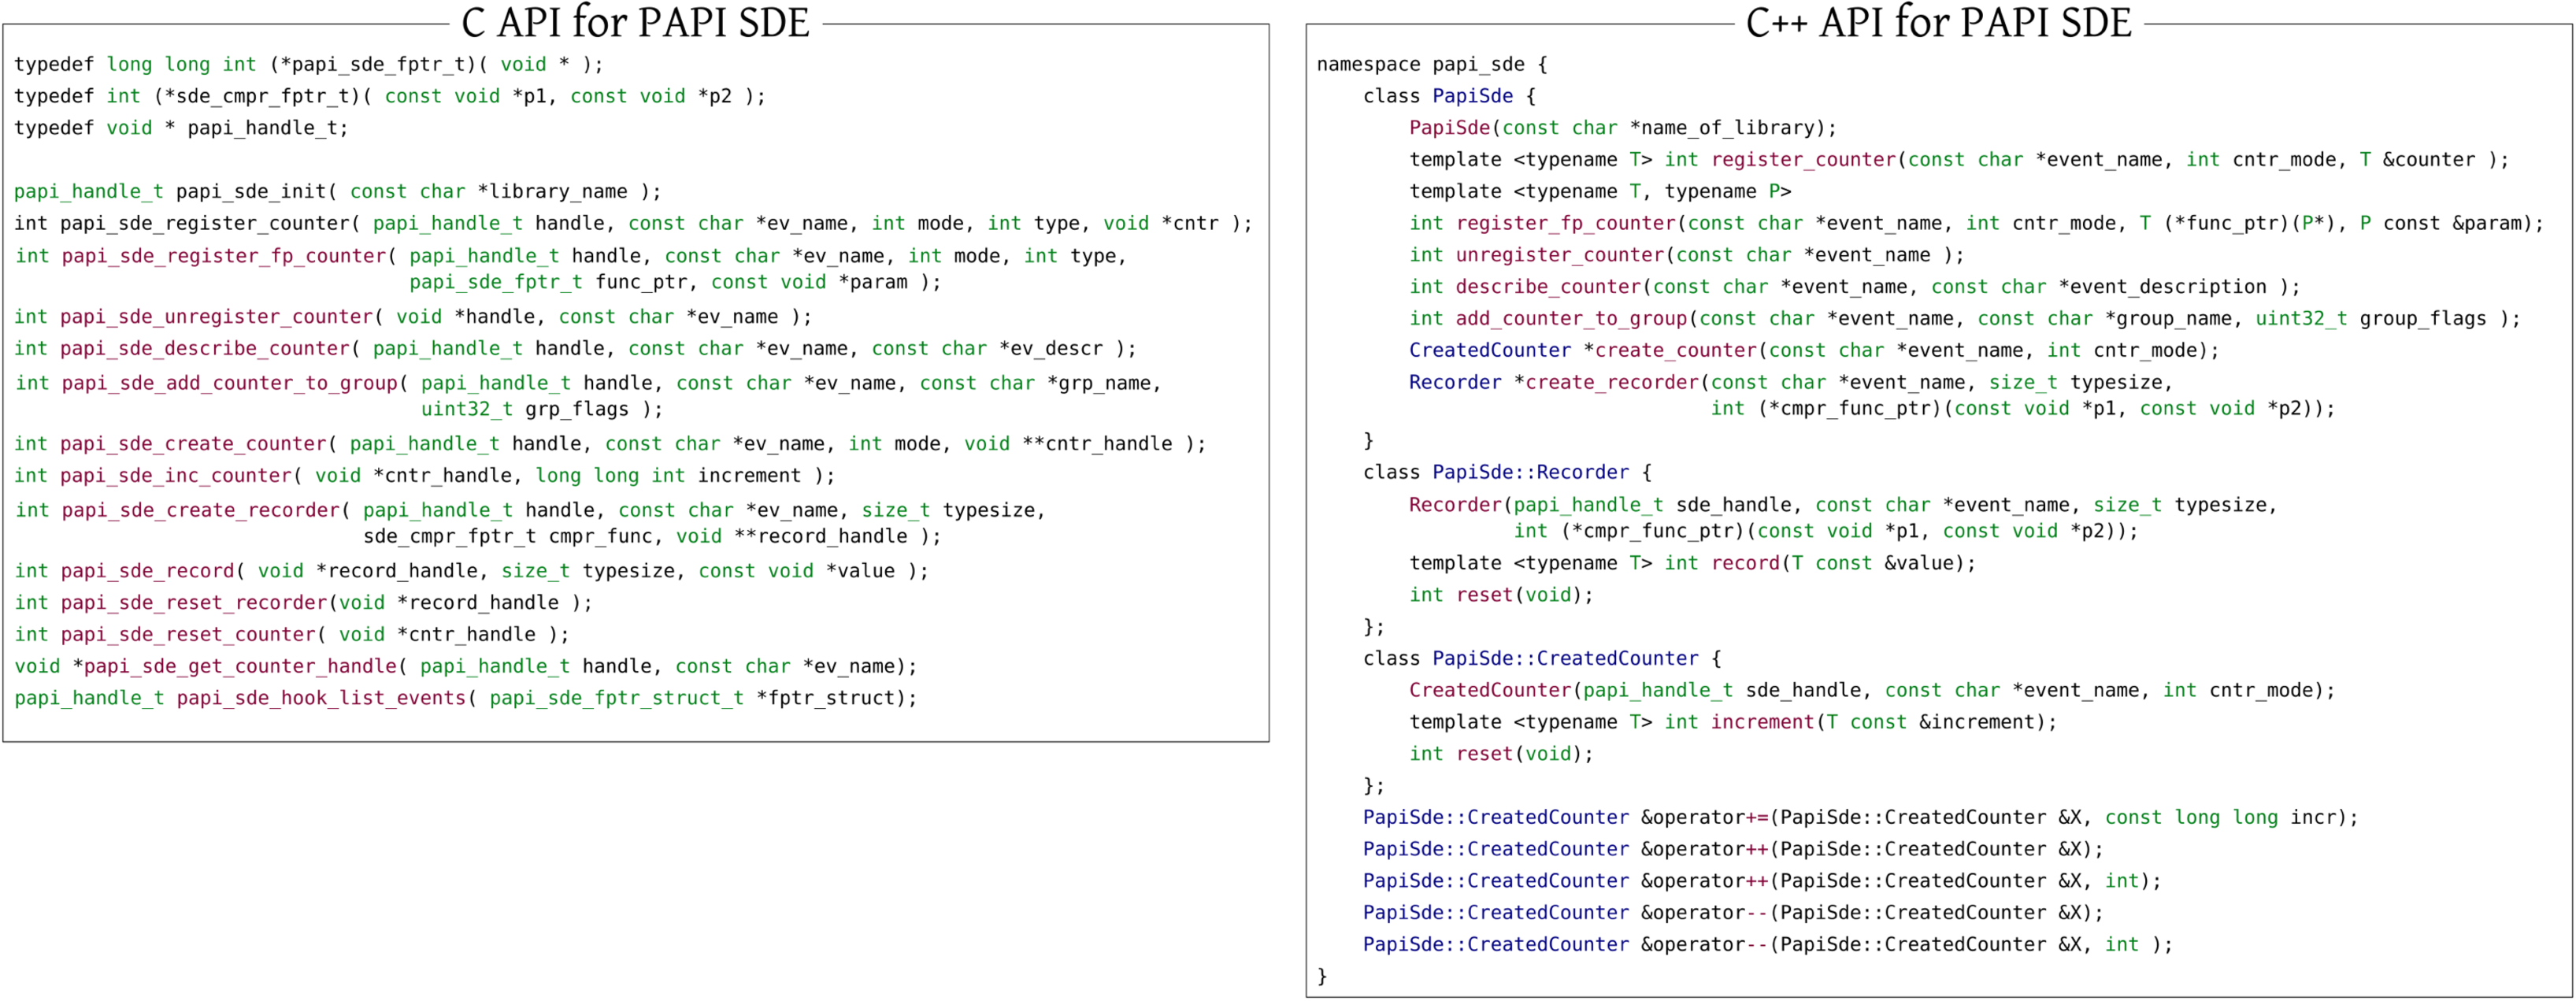
\includegraphics[width=0.88\linewidth]{projects/2.3.2-Tools/2.3.2.06-EXA-PAPI/papi_sde.pdf}
\caption{Existing PAPI SDE C API and new SDE C++ API.}
\label{fig:papi_sde}
\end{center}
\end{figure}


\paragraph{Recent Progress}

The Exa-PAPI team is in the process to prepare a major release---PAPI 7.0.0---scheduled
to be shipped in November 2021. For this release, the team has  
designed and developed a C++ API for utilizing PAPI's software-defined events (SDEs) 
from within third-party libraries and applications that are written in C++. 
This is a major addition to the already implemented and released 
C and FORTRAN APIs for the PAPI SDE functionality (shipped with PAPI 6.0.0 in 
March 2020). The example code in Figure~\ref{fig:papi_sde} demonstrate  the 
C and C++ API for PAPI SDEs. 
%

\vspace{10pt}
Furthermore, PAPI 7.0.0 will release newly developed support for the latest monitoring
features on the Intel Gen9 GPUs. 
This was accomplished under NDA and in very close collaboration with the Intel team. 
The new PAPI capabilities for monitoring Intel Gen9 include GPU hardware 
events, and memory performance metrics (bytes read/written/transferred from/to L3).
Monitoring of GPU and memory performance counters aids developers in producing
more efficient code by profiling the utilization of the latest GPU resources and
diagnosing performance bottlenecks.
The objective of this development was to  
%a mechanism to collect Intel
%GPU performance metrics via PAPI�s well known interface and without any additional
%efforts from the users.
%In our approach, through the PAPI component framework, we 
enable transparent access
to the Gen9 performance and memory metrics via Intel's OneAPI Level-Zero Interface.
A unique feature of this development enables users to apply two different collection modes 
via the PAPI interface:\\
The Time-based Collection Mode:
\begin{itemize}
\item Counter values are aggregated and stored in a buffer.
\item Counter values can be read at any given time during the execution, which means
performance counter monitoring is completely autonomous from the kernels
running in the GPUs.
\end{itemize}
%
The Kernel-based Collection Mode:
\begin{itemize}
\item Counter monitoring is per kernel.
\item Performance counter data is not available during kernel execution but only after
the kernel finishes.
\item In this mode, the Level-Zero API uses internal barriers, which implies, if two
kernels overlap, the execution of the second kernel is pushed out until the first
kernel finishes.
\end{itemize}


\vspace{10pt}
Another major change in PAPI 7.0.0 is the refactoring of the PAPI CUDA component and 
new developments to support NVIDIA compute capability 7.0 and greater. This required
the use of the CUDA/CUPTI 11 Profiling and Perfworks APIs. The PAPI CUDA component 
has been redesigned so that it works in equal measure for NVIDIA compute capabilities 
$<$ 7.0 and $\geq$ 7.0. 
 
 
 \vspace{10pt}
Last but not least, the team designed and implemented PAPI support for FUGAKU's A64FX 
Arm architecture. This work includes the development of new Counter Analysis Toolkit (CAT) 
benchmarks and refinements of PAPI's CAT data analysis; specifically, the extension of 
PAPI's CAT with MPI and ``distributed memory''-aware benchmarks and analysis in order to 
stress all cores/node. The CAT analysis of the A64FX raw hardware counters resulted in the 
definition of 36 new PAPI presets for FUGAKU users.
 
 

\paragraph{Next Steps}

Our next efforts will focus on:
\begin{enumerate}
\item \textbf{Modernize atomics and reduce overhead in PAPI:} 
	When PAPI calls are made from within different thread contexts, PAPI uses internal 
	mechanisms for guaranteeing thread safety. 
	Atomic operations have a central role in these mechanisms, since they introduce less 
	overhead than mutexes. 
	However, the support for atomic operations in the current PAPI framework is limited, 
	and many opportunities are missed. Projects such as ``the atomic\_ops library'' offer a 
	much wider support for atomic operations, which the team plans to leverage in PAPI.

%
\item \textbf{Improved multi-threading and OpenMP support in PAPI}: 
	Beyond the atomic operations for guaranteeing correctness, PAPI will modernize 
	support for threads. PAPI was originally designed in a time when threads were exotic, 
	and OpenMP was nonexistent. The Exa-PAPI team will improve the interoperability with 
	thread systems and OpenMP in particular.

%
\item \textbf{Development of PAPI support for new ECP hardware}:
	Development of new PAPI components, as well as new features in current PAPI 
	components due to underlying vendor interface updates. Development of new PAPI 
	presets (predefined events) for newly released hardware.
\end{enumerate}
